\chapter{\MakeUppercase{Connection with Optimization}}

\section{Newton-Type Methods and Optimization}

Nonlinear equation solving and optimization are closely related areas in numerical mathematics. Although the primary objective of root-finding methods is to solve equations of the form
\[
f(x)=0
\]
or
\[
F(\mathbf{x})=\mathbf{0},
\]
many iterative algorithms can also be interpreted from an optimization perspective \cite{nocedal, kelley}.

For a scalar nonlinear equation, solving
\[
f(x)=0
\]
can be reformulated as minimizing a residual-based objective function. One common choice is the merit function
\[
\phi(x)=\frac{1}{2}|f(x)|^2.
\]

The factor
\[
\frac{1}{2}
\]
is introduced mainly for notational convenience when derivatives are computed.

If
\[
x^\ast
\]
is an exact root of the nonlinear equation, then
\[
f(x^\ast)=0,
\]
which immediately gives
\[
\phi(x^\ast)=0.
\]

Therefore, every exact root of the equation corresponds to a global minimizer of the merit function.

A similar formulation can also be constructed for nonlinear systems. Consider the system
\[
F(\mathbf{x})=\mathbf{0},
\]
where
\[
F:\mathbb{R}^n\to\mathbb{R}^n.
\]

The corresponding merit function is defined as
\[
\phi(\mathbf{x})
=
\frac{1}{2}
\|F(\mathbf{x})\|^2.
\]

Using the Euclidean norm,
\[
\|F(\mathbf{x})\|^2
=
F(\mathbf{x})^T F(\mathbf{x}),
\]
the objective function becomes
\[
\phi(\mathbf{x})
=
\frac{1}{2}
F(\mathbf{x})^T F(\mathbf{x}).
\]

This formulation transforms the nonlinear equation problem into an unconstrained optimization problem \cite{nocedal}.

The optimization viewpoint becomes especially useful when direct root-finding iterations behave unstably or when exact roots are difficult to compute. In such situations, instead of forcing the residual to become exactly zero at every step, the algorithm attempts to reduce the residual function gradually.

The connection between Newton's method and optimization can also be seen directly from the iteration formula itself. Consider the optimization problem
\[
\min \phi(x).
\]

A stationary point satisfies
\[
\phi'(x)=0.
\]

Applying Newton's method to this optimization problem gives the iteration
\[
x_{k+1}
=
x_k
-
\frac{\phi'(x_k)}{\phi''(x_k)}.
\]

Now consider the merit function
\[
\phi(x)
=
\frac{1}{2}f(x)^2.
\]

The first derivative is
\[
\phi'(x)
=
f(x)f'(x),
\]
while the second derivative becomes
\[
\phi''(x)
=
[f'(x)]^2
+
f(x)f''(x).
\]

Substituting these expressions into Newton's optimization formula gives
\[
x_{k+1}
=
x_k
-
\frac{
f(x_k)f'(x_k)
}{
[f'(x_k)]^2
+
f(x_k)f''(x_k)
}.
\]

Near the root,
\[
f(x_k)
\]
becomes small, and therefore the term
\[
f(x_k)f''(x_k)
\]
can often be neglected locally. This approximation leads to
\[
x_{k+1}
\approx
x_k
-
\frac{f(x_k)}{f'(x_k)},
\]
which is precisely the classical Newton iteration for nonlinear equations.

This interpretation shows that Newton's method can be viewed not only as a root-finding algorithm but also as an optimization-inspired method that minimizes the residual function locally \cite{kelley, nocedal}.

\section{Line Search and Armijo Condition}

Although Newton's method converges very rapidly near the solution, the method may behave unstably when the initial approximation is not sufficiently close to the root. In some cases, the full Newton step may become excessively large and cause divergence or oscillatory behavior \cite{kelley}.

To improve stability, optimization algorithms often use line-search strategies. Instead of accepting the full iteration step immediately, the algorithm searches for a suitable step size that decreases the objective function sufficiently.

For nonlinear equation solving, consider the Newton direction
\[
s_k
=
-
\frac{f(x_k)}{f'(x_k)}.
\]

Instead of using the full update
\[
x_{k+1}=x_k+s_k,
\]
a damped iteration is constructed:
\[
x_{k+1}
=
x_k+\alpha_k s_k,
\]
where
\[
0<\alpha_k\leq1
\]
is the step-size parameter.

The value of
\[
\alpha_k
\]
is selected in such a way that the merit function decreases sufficiently. One of the most widely used criteria for this purpose is the Armijo condition \cite{nocedal}.

Using the merit function
\[
\phi(x)=\frac{1}{2}f(x)^2,
\]
the Armijo condition is written as
\[
\phi(x_k+\alpha_k s_k)
\leq
\phi(x_k)
+
c\,\alpha_k\,\phi'(x_k)s_k,
\]
where
\[
0<c<1
\]
is a small positive constant.

The purpose of this condition is to guarantee sufficient decrease of the merit function at every iteration. Instead of accepting any arbitrary step, the algorithm only accepts updates that produce meaningful improvement in the residual.

In practice, the step size is usually determined using a backtracking strategy. The process starts with
\[
\alpha_k=1,
\]
which corresponds to the full Newton step. If the Armijo condition is not satisfied, the step size is reduced repeatedly:
\[
\alpha_k \leftarrow \rho \alpha_k,
\]
where
\[
0<\rho<1
\]
is a reduction factor, typically chosen as
\[
\rho=0.5.
\]

This procedure continues until the Armijo condition becomes satisfied.

The overall strategy provides a balance between convergence speed and numerical stability. Near the solution, the algorithm often accepts the full Newton step and preserves rapid convergence. Far from the solution, smaller step sizes improve robustness and reduce the risk of divergence \cite{nocedal, kelley}.

Line-search techniques and Armijo-type conditions are widely used in optimization algorithms, particularly in Newton and quasi-Newton methods. Similar ideas can also be applied naturally to nonlinear equation solving because both problems rely heavily on controlling iterative updates.

\paragraph{Implementation Example.}

The following implementation fragment shows the main computational structure of the adaptive damped Newton method. The step size is first set to one, and then it is reduced by backtracking until the Armijo condition is satisfied.

\begin{lstlisting}
def adaptive_damped_newton(
    f, df, x0,
    tol=1e-8,
    max_iter=100,
    c=1e-4,
    rho=0.5
):

    def phi(x):
        return 0.5 * f(x) ** 2

    x = x0
    history = []

    for i in range(max_iter):

        fx = f(x)
        dfx = df(x)

        if abs(dfx) < 1e-15:
            raise ValueError("Derivative is too small.")

        step_direction = -fx / dfx
        alpha = 1.0

        phi_x = phi(x)
        phi_prime_x = fx * dfx

        while (
            phi(x + alpha * step_direction)
            > phi_x + c * alpha * phi_prime_x * step_direction
        ):
            alpha *= rho

        x_next = x + alpha * step_direction

        history.append({
            "iteration": i,
            "x": x,
            "alpha": alpha,
            "residual": abs(fx)
        })

        if abs(f(x_next)) <= tol:
            return x_next, history

        x = x_next

    return x, history
\end{lstlisting}

\section{Adaptive Damped Newton Method}

The classical damped Newton method introduces a constant damping parameter in order to stabilize the iteration process. However, using a fixed step size may be inefficient because the same damping factor is applied throughout the entire computation, regardless of the local behavior of the function.

An adaptive damping strategy attempts to overcome this limitation by adjusting the step size dynamically during the iteration process.

Consider again the Newton direction
\[
s_k
=
-
\frac{f(x_k)}{f'(x_k)}.
\]

Instead of using a constant damping parameter, the adaptive damped Newton method computes the iteration
\[
x_{k+1}
=
x_k+\alpha_k s_k,
\]
where
\[
\alpha_k
\]
is selected automatically using a line-search procedure.

In this study, the step size is determined using a backtracking Armijo strategy. The algorithm first attempts the full Newton step with
\[
\alpha_k=1.
\]

If the resulting update does not satisfy the Armijo condition, the step size is reduced repeatedly until sufficient decrease of the merit function is achieved.

This adaptive mechanism allows the method to behave differently depending on the current region of the function. Near the root, the method often accepts large step sizes and preserves the fast convergence properties of Newton's method. In more unstable regions, the algorithm automatically reduces the step length in order to maintain stability.

Compared to the constant damped Newton method, the adaptive version generally provides better balance between robustness and convergence speed. Instead of relying on a manually selected damping parameter, the algorithm adjusts itself according to the local behavior of the residual function.

The adaptive damped Newton method also demonstrates the strong connection between nonlinear equation solving and optimization algorithms. The use of merit functions, sufficient decrease conditions, and backtracking procedures directly follows ideas commonly used in modern optimization theory \cite{nocedal}.

In the next section, numerical experiments are presented in order to compare the behavior of the classical Newton method, the constant damped Newton method, and the adaptive Armijo-based damped Newton method.

\section{Numerical Experiments}

In order to examine the practical effect of Armijo-based damping, an additional numerical experiment was carried out. The purpose of this experiment is to compare three Newton-type methods under the same initial condition:

\begin{itemize}
    \item classical Newton's method,
    \item constant damped Newton's method,
    \item adaptive Armijo-based damped Newton's method.
\end{itemize}

The nonlinear equation used in this experiment is
\[
f(x)=\tan(x)-x-1.
\]

Its derivative is
\[
f'(x)=\sec^2(x)-1.
\]

Equivalently, in computational form, this derivative can be written as
\[
f'(x)=\frac{1}{\cos^2(x)}-1.
\]

This function was selected because it is nonlinear, transcendental, and sensitive to the choice of the initial approximation. The tangent function may change rapidly near its vertical asymptotes, and this makes the problem useful for observing the stabilizing effect of line-search techniques. In other words, the example is not chosen only because it has a root, but because it can expose the difference between an uncontrolled Newton step and an adaptively controlled one.

The initial approximation was chosen as
\[
x_0=0.5.
\]

This starting point is deliberately not very close to the root. From this value, the full Newton step becomes too aggressive and the classical Newton method moves away from the solution. Therefore, this initial value is suitable for showing why step-size control is needed.

For the constant damped Newton method, the damping parameter was fixed as
\[
\alpha=0.25.
\]

This value was chosen because it is small enough to stabilize the iteration, but it also makes the method noticeably slower. This allows the experiment to show the main weakness of constant damping: the method may be safe, but it can lose too much speed.

For the adaptive method, the step size
\[
\alpha_k
\]
was not fixed in advance. Instead, it was selected at each iteration using the Armijo backtracking strategy. The method first tried the full Newton step. If the Armijo condition was not satisfied, the step size was reduced until sufficient decrease of the merit function was obtained.

Figure~\ref{fig:armijo_residual_comparison} shows the residual behavior of the three methods.

\begin{figure}[h!]
\centering

\includegraphics[width=0.85\textwidth]{figures/armijo_residual_comparison.png}
\caption{Residual comparison of Newton-type methods}
\label{fig:armijo_residual_comparison}
\end{figure}

The results show that the classical Newton method fails for this initial value. The residual grows very rapidly and the method does not converge within the allowed number of iterations. This behavior occurs because the full Newton step is accepted at every iteration, even when the step does not reduce the residual.

The constant damped Newton method behaves more safely. Since the step size is fixed at
\[
\alpha=0.25,
\]
the method avoids the large unstable steps observed in the classical Newton method. However, this stability comes with a cost. The residual decreases slowly, and the method requires many iterations before convergence.

The adaptive Armijo-based method gives a better balance. At the beginning of the iteration, the method reduces the step size in order to avoid instability. After the iterates move into a more reliable region, the method accepts larger steps and reaches the root much faster.

The root obtained by both convergent methods is approximately
\[
x^\ast \approx 1.132268.
\]

Figure~\ref{fig:armijo_alpha_history} shows the step sizes selected by the Armijo backtracking procedure.

\begin{figure}[h!]
\centering
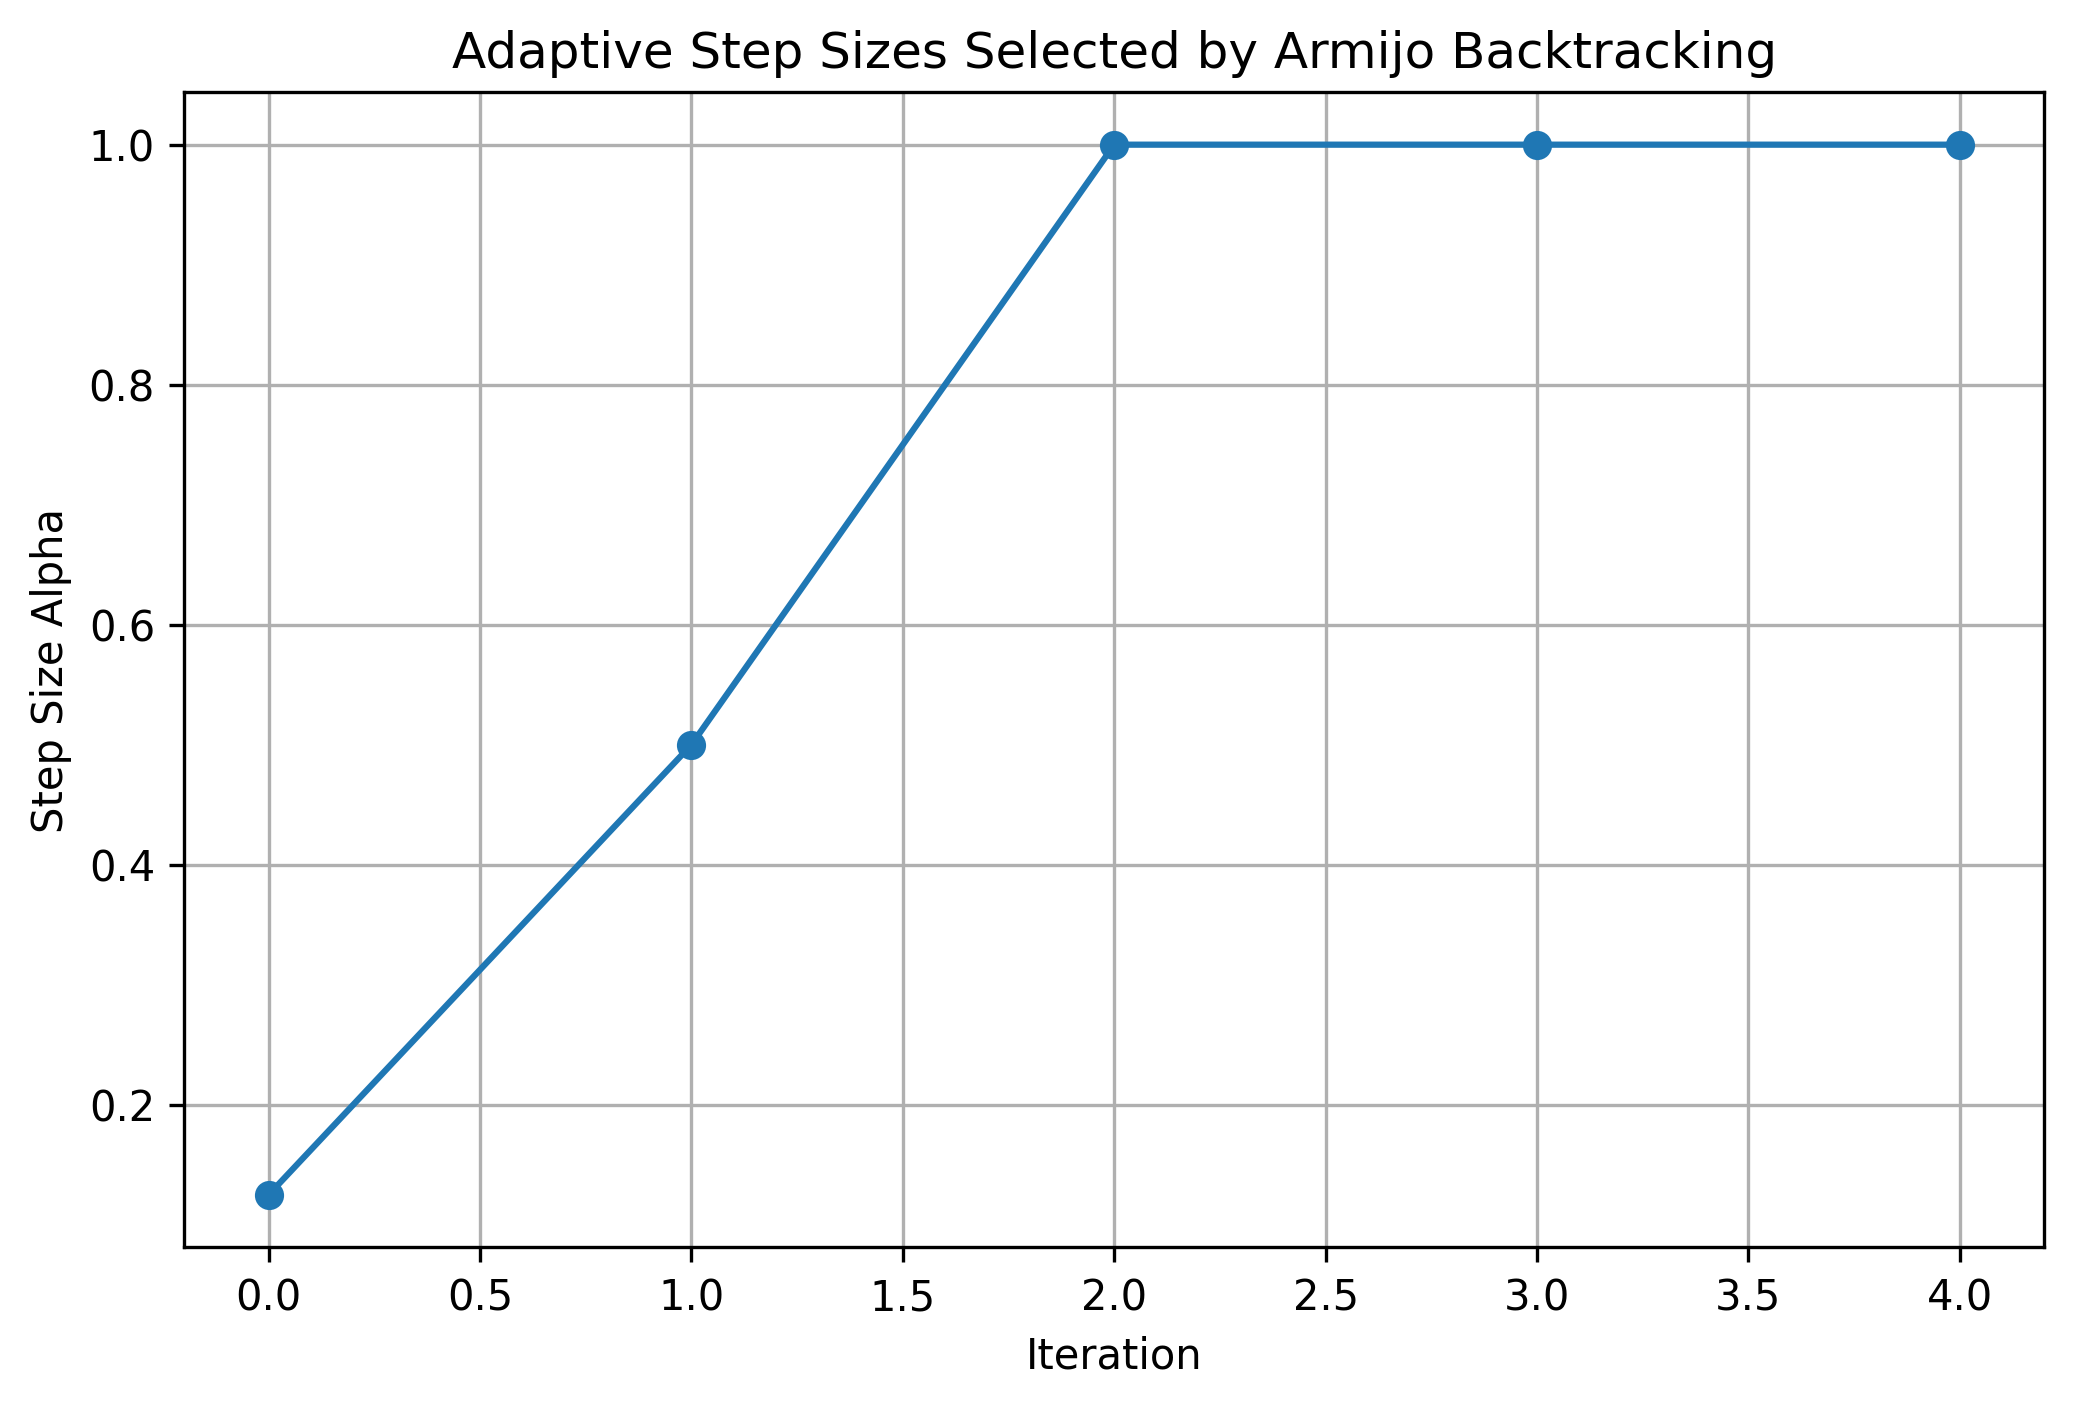
\includegraphics[width=0.75\textwidth]{figures/armijo_alpha_history.png}
\caption{Adaptive step sizes selected by Armijo backtracking}
\label{fig:armijo_alpha_history}
\end{figure}

The step-size plot shows the adaptive character of the method clearly. In the first iteration, the algorithm selects a small value of
\[
\alpha_k.
\]
This prevents the method from taking an unstable full Newton step. In the later iterations, the selected step size increases. Once the iterates are close enough to the root, the method accepts
\[
\alpha_k=1,
\]
which corresponds to the full Newton step.

Table~\ref{tab:armijo_comparison} summarizes the numerical results.

\begin{table}[h!]
\centering
\caption{Comparison of Newton-type methods with Armijo stabilization}
\label{tab:armijo_comparison}
\begin{tabular}{|c|c|c|c|}
\hline
Method & Iterations & Final Residual & Converged \\ \hline
Newton & 75 & \(4.45\times10^{40}\) & No \\ \hline
Constant Damped Newton & 58 & \(1.15\times10^{-7}\) & Yes \\ \hline
Adaptive Armijo Newton & 5 & \(3.06\times10^{-9}\) & Yes \\ \hline
\end{tabular}
\end{table}

The comparison shows the advantage of adaptive damping. Classical Newton's method is fast only when the full step is reliable. Constant damping improves stability, but it uses the same step size at every iteration and therefore converges slowly. The Armijo-based method adjusts the step size according to the behavior of the merit function. For this reason, it can avoid unstable steps at the beginning and still recover the fast local behavior of Newton's method near the solution.

This experiment supports the main idea of this chapter: optimization-based line-search methods are not only theoretical tools, but they can also improve the practical behavior of nonlinear equation solvers.

\section{Discussion}

The experiments presented in this chapter demonstrate that the practical behavior of Newton-type methods depends strongly on step-size control and stabilization strategies.

Classical Newton's method is known for its very rapid local convergence. When the initial approximation is sufficiently close to the root and the Newton direction is reliable, the method usually converges within only a few iterations. However, the numerical experiments showed that the method may also become highly unstable when these conditions are not satisfied. In the selected test problem, the full Newton step produced excessively large updates and caused divergence.

The constant damped Newton method improved stability by restricting the step size. The smaller updates prevented the divergence observed in the classical Newton iteration. Nevertheless, the use of a fixed damping parameter also introduced an important disadvantage. Since the same step size was used throughout the entire iteration process, the method converged much more slowly, even after the iterates entered a stable region near the root.

The adaptive Armijo-based method provided a more balanced behavior. Instead of relying on a fixed damping parameter, the algorithm adjusted the step size according to the local behavior of the merit function. During unstable stages of the iteration, the method selected smaller step sizes in order to maintain sufficient decrease of the residual. Once the iterates approached the solution, the algorithm accepted larger step sizes and recovered the fast convergence behavior of Newton's method.

These observations highlight one of the central ideas connecting optimization and nonlinear equation solving. In both areas, the quality of the search direction alone is often insufficient. Controlling the length of the iteration step is equally important for obtaining stable and efficient numerical behavior.

The experiments also demonstrate that optimization-inspired techniques such as merit functions, line-search procedures, and Armijo conditions can significantly improve the robustness of nonlinear solvers. Although these ideas originate mainly from optimization theory, they naturally extend to root-finding problems because both approaches depend heavily on iterative reduction of residuals.

Overall, the adaptive damped Newton method illustrates how optimization-based stabilization strategies can improve nonlinear equation solving without completely sacrificing the rapid local convergence properties of Newton's method.